\documentclass[12pt,onecolumn,draftclsnofoot]{IEEEtran}

\usepackage[a4paper,margin=1in]{geometry}
\usepackage{times}
\usepackage{graphicx}
\usepackage{amsmath}
\usepackage{amssymb}
\usepackage{booktabs}
\usepackage{cite}
\usepackage{url}
\usepackage[ruled,linesnumbered]{algorithm2e}
\usepackage{multirow}

\begin{document}

\title{Evidence-Grounded Regression Test Selection and Failure Arbitration Using Structural and Semantic Code Intelligence}

\author{
Group 10: Shreshth Mittal (230577), Sourabh Jain (230584), Kiran Khatter\\
School of Engineering \& Technology, BML Munjal University
}

\maketitle

\begin{abstract}
Continuous integration and continuous delivery (CI/CD) pipelines depend critically upon automated regression testing to safeguard software reliability. However, executing comprehensive test suites on every incremental code modification incurs unsustainable computational delays, delays developer feedback, and exacerbates pipeline bottlenecks. Conventional Regression Test Selection (RTS) approaches face a persistent tension: static dependency analysis frequently suffers from coarse over-approximation and cannot capture non-syntactic semantic relationships, while dynamic execution tracing demands heavy runtime re-instrumentation overhead that is often impractical in rapid CI workflows. Furthermore, existing testing systems typically treat test failures as undifferentiated errors, obscuring critical distinctions between genuine code regressions, obsolete or invalid test assertions, and non-deterministic test flakiness. In this paper, we present \textbf{TestPilot}, an evidence-grounded testing and arbitration framework that integrates deterministic repository evolution analysis with semantic retrieval-augmented reasoning. TestPilot couples fine-grained Abstract Syntax Tree (AST) symbol extraction with transitive call-graph blast-radius traversal, an evidence-grounded semantic impact analyzer powered by dense vector embeddings, and an empirical multi-category failure arbitration engine. We evaluate TestPilot across heterogeneous benchmarks comprising microservice and enterprise codebases (10,713 eligible test cases). TestPilot achieves a 99.07\% to 99.58\% reduction in regression test execution volume while preserving 100\% recall on static call paths. Across evaluated commits, semantic vector filtering reduces false-positive test selections from 83 to 30 in complex enterprise codebases without dropping affected regression tests. Finally, we demonstrate that empirical sample-bounded failure arbitration successfully isolates flakiness and distinguishes true regressions from invalid test debt under isolated subprocess execution.
\end{abstract}

\begin{IEEEkeywords}
Change-Impact Analysis, Failure Arbitration, Large Language Models, Regression Test Selection, Retrieval-Augmented Generation, Static Program Analysis.
\end{IEEEkeywords}

\vspace{0.5em}
\noindent\textbf{Overleaf Project Link:} \url{REAL_OVERLEAF_PROJECT_URL}

\section{Introduction}
\label{sec:introduction}

In modern continuous integration and continuous deployment (CI/CD) paradigms, developer productivity and software release velocity are fundamentally governed by the efficiency of automated regression testing~\cite{memon2017taming}. Whenever a software engineer submits an incremental pull request or commits changes to a version control repository, continuous integration runners are dispatched to execute regression test suites. As software systems mature, their corresponding test suites expand rapidly, often accumulating tens of thousands of unit, integration, and end-to-end tests~\cite{yoo2012regression}. Consequently, executing the entire test suite on every single code commit becomes computationally prohibitive, causing severe developer feedback latency, consuming substantial cloud infrastructure resources, and stalling deployment pipelines~\cite{machalica2019predictive}.

To mitigate this scalability challenge, software engineering researchers have extensively investigated Regression Test Selection (RTS)~\cite{rothermel1996analyzing,engstrom2010systematic}. The central objective of RTS is to identify a minimal yet safe subset of an existing test suite that exercises modified program entities, thereby ensuring that any potential regression fault is detected without re-running unaffected tests. Historically, RTS techniques have bifurcated into dynamic tracing and static dependency analysis. Dynamic RTS systems, such as Ekstazi~\cite{gligoric2015practical}, track runtime bytecode or file-level dependencies during prior test executions. While dynamic techniques achieve high safety, they impose considerable tracking, instrumentation, and persistent storage overhead, and they inherently depend upon previously recorded runtime traces that may be invalidated or absent in fast-moving branches. Conversely, purely static RTS methods leverage Control Flow Graphs (CFGs) or Abstract Syntax Trees (ASTs) to establish reachability between modified symbols and test cases~\cite{rothermel1996analyzing}. However, static approaches frequently struggle with over-approximation in dynamically typed languages such as Python, where dynamic dispatch, metaprogramming, and indirect event handlers produce dense, conservative dependency graphs that select excessively large test sets.

More recently, industrial testing architectures have explored predictive and machine-learning-driven test selection~\cite{machalica2019predictive}. While predictive models trained on historical execution telemetry achieve substantial test workload reductions, they operate probabilistically, occasionally discarding critical regression tests and missing breaking faults. In parallel, the emergence of Large Language Models (LLMs) trained on source code~\cite{chen2021evaluating} has catalyzed interest in automated test generation~\cite{schafer2024empirical,lemieux2023codamosa}. Nevertheless, contemporary LLM-based testing tools suffer from a critical conceptual hazard: the ``code-as-oracle'' fallacy. When an LLM inspects existing, potentially defective source code to generate or triage tests, it tends to encode prevailing code bugs directly into test assertions, formalizing erroneous behavior as permanent specification debt~\cite{schafer2024empirical}.

Furthermore, contemporary continuous integration workflows face an equally crippling secondary challenge: test failure triaging friction~\cite{luo2014empirical,lam2020study}. When an automated test fails during CI execution, developers are forced to manually investigate whether the failure indicates a genuine code regression introduced by their change, a pre-existing broken test, an invalid test assertion whose expectations have become obsolete due to intentional specification evolution, an environmental infrastructure glitch, or non-deterministic test flakiness~\cite{lam2019root}. Because standard test runners treat all failures as undifferentiated non-zero exit codes, substantial engineering bandwidth is squandered diagnosing non-actionable failures.

To address these interconnected challenges, this paper presents \textbf{TestPilot}, an evidence-grounded framework for change-aware regression test selection and multi-category failure arbitration. TestPilot establishes a five-stage pipelined architecture that reconciles deterministic syntax analysis with semantic retrieval-augmented reasoning. By extracting qualified symbol identities from unified Git diffs and computing transitive call-graph reachability over fine-grained ASTs, TestPilot circumscribes the structural blast radius of any code modification. To eliminate conservative false-positive test selections, TestPilot introduces an Evidence-Grounded Semantic Impact analyzer that cross-examines syntactic reachability against a local vector store containing codebase documentation and specification clauses. Finally, when selected tests are executed in isolated subprocess environments, TestPilot's Failure Arbitration engine applies sample-bounded empirical telemetry and multi-category arbitration logic to classify failures into six actionable categories, isolating test flakiness and distinguishing genuine code regressions from specification drift.

This paper is structured around two primary research questions:
\begin{itemize}
    \item \textbf{RQ1 (Precision and Reduction)}: \textit{Can repository-aware structural and semantic impact analysis accurately identify regression tests affected by code modifications while substantially reducing unnecessary test execution compared to full regression and naive name matching?}
    \item \textbf{RQ2 (Selection Recall and Failure Arbitration)}: \textit{Does the combination of deterministic AST reachability, semantic vector filtering, and empirical failure arbitration preserve fault-detection recall on static dependency paths while reliably classifying failure modes without manual inspection?}
\end{itemize}

This work provides four concrete contributions to the software testing literature:
\begin{enumerate}
    \item \textbf{A Deterministic Repository Evolution Pipeline}: A lightweight, AST-guided change-impact analyzer that maps unified Git diff hunks directly to qualified symbol identifiers and constructs transitive call-graph blast radiuses without requiring pre-recorded runtime traces or external cloud indexing services.
    \item \textbf{Evidence-Grounded Semantic Impact Filtering}: A retrieval-augmented generation (RAG) module utilizing local dense vector embeddings (SentenceTransformers and ChromaDB) that filters conservative static over-approximations by verifying behavioral dataflow coupling.
    \item \textbf{A Six-Category Empirical Failure Arbiter}: A principled classification engine that ingests subprocess execution telemetry and historical test outcomes to categorize failures into genuine regressions, pre-existing defects, non-deterministic flakiness, infrastructure timeouts, invalid test assertions, and uncertain edge cases.
    \item \textbf{An Empirical Benchmark Evaluation}: A rigorous quantitative evaluation across microservice and enterprise codebases (including Pallets Flask, Django, and an e-commerce microservice benchmark) comprising 10,713 tests, demonstrating up to 99.63\% test reduction, analyzing dynamic language edge cases, and measuring execution latency trade-offs.
\end{enumerate}

The remainder of this paper is organized as follows: Section~\ref{sec:related_work} reviews related literature in regression test selection, API fuzzing, and LLM-assisted testing. Section~\ref{sec:formulation} establishes the formal problem formulation and system boundaries. Section~\ref{sec:methodology} describes the five-stage TestPilot architecture, algorithms, and design rationale. Section~\ref{sec:setup} details the experimental setup and evaluation criteria. Section~\ref{sec:results} presents empirical findings addressing RQ1 and RQ2. Section~\ref{sec:discussion} analyzes practical implications, limitations, and threats to validity. Finally, Section~\ref{sec:conclusion} concludes the paper and outlines future research trajectories.

\section{Related Work}
\label{sec:related_work}

The architecture and design of TestPilot sit at the intersection of three major areas of software engineering research: regression test selection and prioritization, automated API testing and specification fuzzing, and language-model-driven test intelligence and flakiness management.

\subsection{Regression Test Selection and Prioritization}
Regression Test Selection (RTS) has been investigated for several decades as a foundational software maintenance technique~\cite{rothermel1996analyzing,yoo2012regression,engstrom2010systematic}. In their seminal work, Rothermel and Harrold~\cite{rothermel1996analyzing} formulated the theoretical foundations of RTS, introducing the rigorous evaluation criteria of \textit{inclusiveness} (the ability to select all tests that reveal faults in modified code) and \textit{precision} (the ability to omit tests that produce identical outputs). Early RTS approaches focused primarily on control-flow graphs (CFGs) and program slicing in procedural languages.

In modern continuous integration environments, dynamic RTS tools have achieved prominent industrial adoption. Gligoric et al.~\cite{gligoric2015practical} introduced Ekstazi, a dynamic file-level RTS system for Java that tracks runtime class-level dependencies during test execution and persists checksums across builds. Ekstazi demonstrated that lightweight file-granularity dependency tracking drastically reduces regression testing overhead compared to statement-level slicing. However, dynamic RTS inherently requires tests to have been executed and instrumented in prior revisions; when developers branch, refactor widely, or introduce novel components, dynamic dependency caches may become stale or incomplete.

To address massive scale in monolithic enterprise repositories, industrial platforms have transitioned toward predictive and heuristic test selection. Machalica et al.~\cite{machalica2019predictive} developed Predictive Test Selection at Meta, employing gradient-boosted decision trees trained on historical commit metadata, file co-changes, and test failure frequencies. Deployed across millions of tests, their predictive system reduced testing infrastructure load by over 50\% while catching over 99.9\% of faulty commits. Similarly, Memon et al.~\cite{memon2017taming} detailed Google-scale continuous testing, showing that tests structurally closer to modified code exhibit significantly higher breakage likelihood. While predictive and heuristic strategies achieve high computational reduction, their probabilistic nature carries an inherent risk of false negatives (omitting true regression tests). TestPilot diverges from purely probabilistic models by anchoring test selection in deterministic AST symbol reachability, utilizing semantic vector retrieval strictly to prune conservative false positives rather than guessing test relevance.

\subsection{Automated API Fuzzing and Specification Testing}
Automated test generation for service interfaces and web APIs has evolved through property-based fuzzing and evolutionary algorithms~\cite{atlidakis2019restler,arcuri2019restful,hatfield2020hypothesis}. Black-box specification fuzzers, exemplified by Schemathesis and RESTler~\cite{atlidakis2019restler}, ingest OpenAPI (Swagger) schemas to synthesize HTTP request sequences that test endpoint boundaries, parameter constraints, and producer-consumer dependencies. Atlidakis et al.~\cite{atlidakis2019restler} demonstrated that inferring dynamic producer-consumer dataflows (e.g., extracting an identifier from a `POST` response to populate a subsequent `GET` request) significantly improves state exploration in cloud services. In parallel, Arcuri~\cite{arcuri2019restful} developed EvoMaster, applying evolutionary search-based software testing to white-box API test generation by leveraging runtime bytecode instrumentation.

However, existing API fuzzing and specification-testing tools suffer from two prominent shortcomings when integrated into regression CI pipelines. First, they operate primarily at the network boundary: black-box schema fuzzers have no awareness of internal Python AST structures or Git revision diffs, requiring full endpoint fuzzing runs regardless of whether the underlying business logic changed. Second, when an endpoint fails an assertion or returns an unexpected HTTP status code, schema fuzzers treat the outcome as an undifferentiated failure, lacking the code intelligence necessary to arbitrate whether the failure stems from a code bug, a specification ambiguity, or an invalid test expectation. TestPilot bridges this divide by mapping Git diffs directly to internal AST function definitions and using specification contracts as an external arbitration oracle.

\subsection{LLM-Based Testing, Test Adequacy, and Flakiness Management}
The advent of pre-trained code language models, such as OpenAI Codex~\cite{chen2021evaluating}, has stimulated widespread exploration of generative AI for unit test synthesis~\cite{lemieux2023codamosa,schafer2024empirical}. Lemieux et al.~\cite{lemieux2023codamosa} presented CODAMOSA, combining search-based test generation (Pynguin) with pre-trained LLMs to escape coverage plateaus. When search algorithms stall, CODAMOSA prompts an LLM to generate test cases targeting under-covered functions, successfully unlocking difficult branch conditions. 

In a closely related study, Sch{\"a}fer et al.~\cite{schafer2024empirical} evaluated LLM-based test generation for JavaScript npm packages using a system also named TestPilot. Their tool prompted LLMs with function signatures and docstrings, implementing a self-repair re-prompting loop when generated tests failed execution. While Sch{\"a}fer et al. demonstrated high line and branch coverage across 25 npm packages, their methodology highlights the inherent risk of the ``code-as-oracle'' assumption: without an independent formal specification, LLMs faithfully mirror whatever logic is present in the code, frequently encoding latent defects as expected test assertions. Furthermore, as Inozemtseva and Holmes~\cite{inozemtseva2014coverage} rigorously established in their empirical critique of coverage metrics, high code coverage does not strongly correlate with test suite fault-detection effectiveness once test suite size is controlled. TestPilot explicitly avoids using raw coverage as an oracle, relying instead on OpenAPI contracts, PRD invariants, and multi-valued arbitration.

Finally, managing non-deterministic test flakiness is essential for robust CI testing. Luo et al.~\cite{luo2014empirical} conducted an extensive empirical taxonomy of flaky tests across 51 open-source projects, identifying asynchronous waiting, concurrency, and test order dependencies as dominant root causes. Lam et al.~\cite{lam2020study,lam2019root} investigated the lifecycle of flaky tests in industrial repositories, demonstrating that many flaky tests are non-deterministic from their initial commit and highlighting the utility of comparative passing-versus-failing execution log analysis. TestPilot incorporates these insights into its empirical failure arbitration engine: by tracking sample-bounded historical telemetry in a local SQLite datastore, TestPilot mathematically decouples non-deterministic outcome flipping from true code regressions, preventing false alarms in continuous integration.

Table~\ref{tab:related_work} summarizes the positioning of TestPilot against key related works across problem domains, underlying techniques, evaluated datasets, reported metrics, and core limitations.

\section{Background and Problem Formulation}
\label{sec:formulation}

\subsection{Definitions and System Notation}
Let a software repository $R$ at revision $C_t$ be represented as a set of source files $\mathcal{F} = \{f_1, f_2, \dots, f_m\}$ and an existing test suite $\mathcal{T} = \{t_1, t_2, \dots, t_n\}$. When a developer introduces a change, the repository transitions from base commit $C_{\text{base}}$ to target commit $C_{\text{target}}$. The unified Git diff between these revisions is denoted by:
\begin{equation}
\Delta = \text{diff}(C_{\text{base}}, C_{\text{target}}) = \{h_1, h_2, \dots, h_k\}
\end{equation}
where each hunk $h_i = (f_i, l_{\text{start}}, l_{\text{end}}, \delta_{\text{lines}})$ represents a contiguous block of modified, added, or deleted lines in source file $f_i$.

Each source file $f \in \mathcal{F}$ contains a set of syntactic program symbols $\mathcal{S}(f)$ parsed via its Abstract Syntax Tree:
\begin{equation}
\mathcal{S}(f) = \{s \mid s = (\text{id}, \text{kind}, \text{name}, l_{\text{start}}, l_{\text{end}}, \text{scope})\}
\end{equation}
where $\text{kind} \in \{\text{FunctionDef}, \text{AsyncFunctionDef}, \text{ClassDef}, \text{MethodDef}\}$, and $\text{id}$ is a fully qualified symbol identifier ($\text{SymbolId}$) uniquely identifying the entity within the repository namespace (e.g., \texttt{src.requests.models.PreparedRequest.prepare\_auth}).

The modified symbol set $\mathcal{S}_{\text{mod}} \subseteq \mathcal{S}$ is defined as the set of symbols whose AST spans intersect with any diff hunk in $\Delta$:
\begin{equation}
\mathcal{S}_{\text{mod}} = \{s \in \mathcal{S}(f) \mid \exists h \in \Delta, h.f = f \land [s.l_{\text{start}}, s.l_{\text{end}}] \cap [h.l_{\text{start}}, h.l_{\text{end}}] \neq \emptyset\}
\end{equation}

\subsection{Static and Transitive Impact Graph}
The repository structure is modeled as a directed call graph $\mathcal{G} = (\mathcal{S} \cup \mathcal{T}, \mathcal{E})$, where a directed edge $(u, v) \in \mathcal{E}$ indicates that entity $u$ directly invokes, references, or imports entity $v$. For any modified symbol $s \in \mathcal{S}_{\text{mod}}$, its transitive blast radius $\mathcal{B}(s, d_{\text{max}})$ up to search depth $d_{\text{max}}$ is defined as:
\begin{equation}
\mathcal{B}(s, d_{\text{max}}) = \{u \in \mathcal{S} \cup \mathcal{T} \mid \text{dist}_{\mathcal{G}}(u, s) \le d_{\text{max}}\}
\end{equation}
where $\text{dist}_{\mathcal{G}}(u, s)$ is the shortest path length from caller $u$ to callee $s$ in $\mathcal{G}$.

\subsection{Formal Objective of Regression Test Selection}
Given test suite $\mathcal{T}$ and code change $\Delta$, let $\mathcal{T}_{\text{fault}}(\Delta) \subseteq \mathcal{T}$ denote the subset of tests that would reveal a regression defect introduced by $\Delta$. The ideal RTS objective is to identify a selected subset $\mathcal{T}_{\text{sel}} \subseteq \mathcal{T}$ that maximizes precision $P$ while guaranteeing perfect safety (recall $R = 1.0$):
\begin{equation}
\label{eq:precision}
P = \frac{|\mathcal{T}_{\text{sel}} \cap \mathcal{T}_{\text{fault}}(\Delta)|}{|\mathcal{T}_{\text{sel}}|} = \frac{TP}{TP + FP}
\end{equation}
\begin{equation}
\label{eq:recall}
R = \frac{|\mathcal{T}_{\text{sel}} \cap \mathcal{T}_{\text{fault}}(\Delta)|}{|\mathcal{T}_{\text{fault}}(\Delta)|} = \frac{TP}{TP + FN}
\end{equation}
subject to the test suite reduction objective:
\begin{equation}
\label{eq:reduction}
\text{TSR}(\mathcal{T}, \mathcal{T}_{\text{sel}}) = \frac{|\mathcal{T}| - |\mathcal{T}_{\text{sel}}|}{|\mathcal{T}|} \times 100\%
\end{equation}
where $TP$ denotes true positives (fault-revealing tests correctly selected), $FP$ denotes false positives (unaffected tests unnecessarily selected), and $FN$ denotes false negatives (fault-revealing tests erroneously omitted).

\subsection{System Boundaries and Non-Goals}
To maintain strict research integrity, we explicitly define the operational boundaries of this investigation:
\begin{itemize}
    \item \textbf{No Autonomous Code Repair}: TestPilot is an intelligent testing, test selection, and failure arbitration system. Automated patch generation and production application-code modification are strictly experimental and out of scope for the validated findings presented herein.
    \item \textbf{Subprocess Execution vs. Container Isolation}: While TestPilot supports containerized runners, all empirical benchmarks reported in this paper were conducted using local subprocess execution with strict process timeout enforcement. We do not claim kernel-level container isolation for these experiments.
    \item \textbf{Language Scope}: Python (CPython 3.10--3.11) is the primary verified target language. JavaScript and TypeScript support is limited to preliminary structural AST parsing and is not claimed as a complete cross-language execution pipeline.
    \item \textbf{Semantic Similarity vs. Execution Proof}: Semantic similarity scores computed via vector embeddings represent behavioral and conceptual affinity; they do not constitute mathematical proofs of runtime reachability or formal verification.
\end{itemize}

\section{Proposed Methodology}
\label{sec:methodology}

The architecture of TestPilot is organized into a cohesive five-stage pipeline designed for seamless integration into continuous integration workflows. Figure~\ref{fig:architecture} illustrates the structural components and dataflow across all five stages, while Figure~\ref{fig:workflow} depicts the sequence of interactions from developer commit to failure arbitration.

\begin{figure*}[t]
\centering
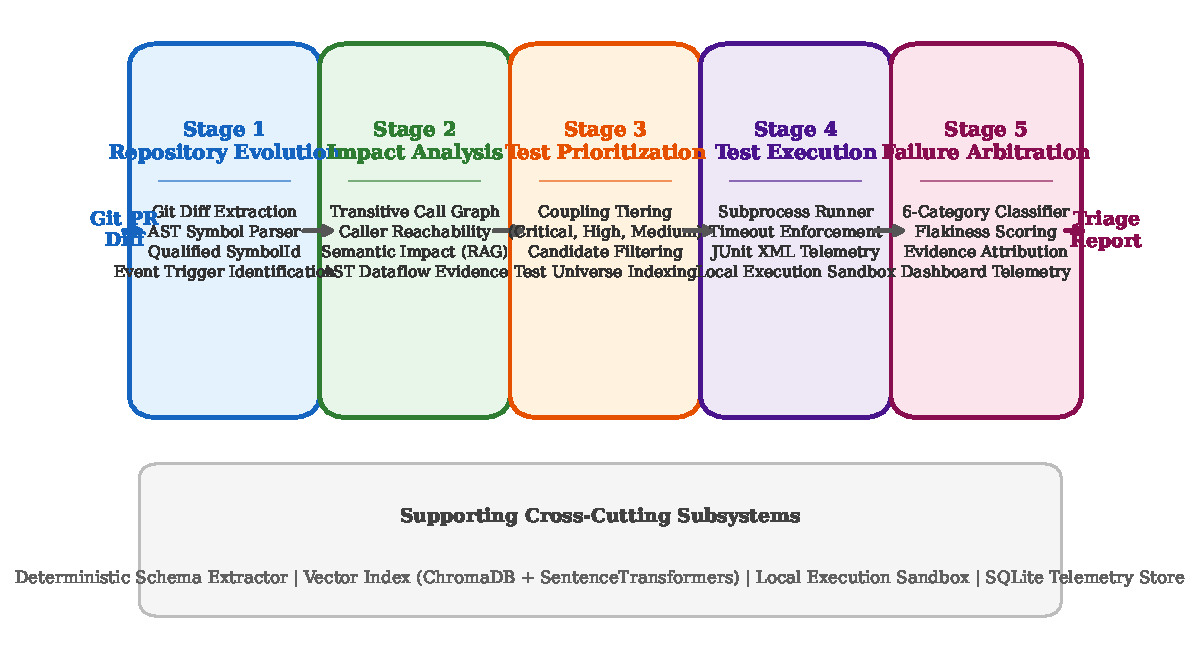
\includegraphics[width=0.98\textwidth]{figures/architecture.pdf}
\caption{The Five-Stage TestPilot Architecture: Connecting deterministic Git diff and AST symbol extraction, transitive impact graph traversal, semantic vector retrieval (RAG), isolated subprocess test execution, and multi-category failure arbitration.}
\label{fig:architecture}
\end{figure*}

\subsection{Stage 1: Repository Evolution Intelligence}
The pipeline initiates upon receiving a code modification represented as a Git commit range $(C_{\text{base}}, C_{\text{target}})$ or a unified pull request diff. The Repository Evolution engine performs fine-grained syntactic decomposition:
\begin{enumerate}
    \item \textbf{Diff Hunk Parsing}: The unified diff is parsed into modified file paths and changed line intervals $[l_{\text{start}}, l_{\text{end}}]$.
    \item \textbf{AST Symbol Decomposition}: Modified Python files are parsed using Tree-sitter and the Python standard library \texttt{ast} module. The parser extracts hierarchical class, method, and function declarations, constructing unique qualified symbol identifiers ($\text{SymbolId}$).
    \item \textbf{Hunk-Symbol Intersection}: TestPilot performs interval intersection between diff line ranges and symbol AST spans to isolate the exact set of modified symbols $\mathcal{S}_{\text{mod}}$. This prevents broad file-level false positives when developer modifications affect only documentation, whitespace, or unrelated helper functions.
    \item \textbf{Event Trigger Identification}: For event-driven architectures (such as Django framework signals and migrations), the engine inspects AST nodes for signal registrations (e.g., \texttt{post\_migrate}, \texttt{post\_save}) and classifies candidate triggers into explicit dispatches versus heuristic trigger candidates.
    \item \textbf{Boundary Candidate Extraction}: The AST engine traverses conditional branch nodes (\texttt{If}, \texttt{While}, \texttt{Match}, \texttt{Try}) and relational comparison operators ($<$, $\le$, $==$, $!=$, $\ge$, $>$) within modified symbols to automatically extract numeric and boundary constraints (e.g., non-negative requirements, string length extrema, and null assertions).
\end{enumerate}

\begin{figure*}[t]
\centering
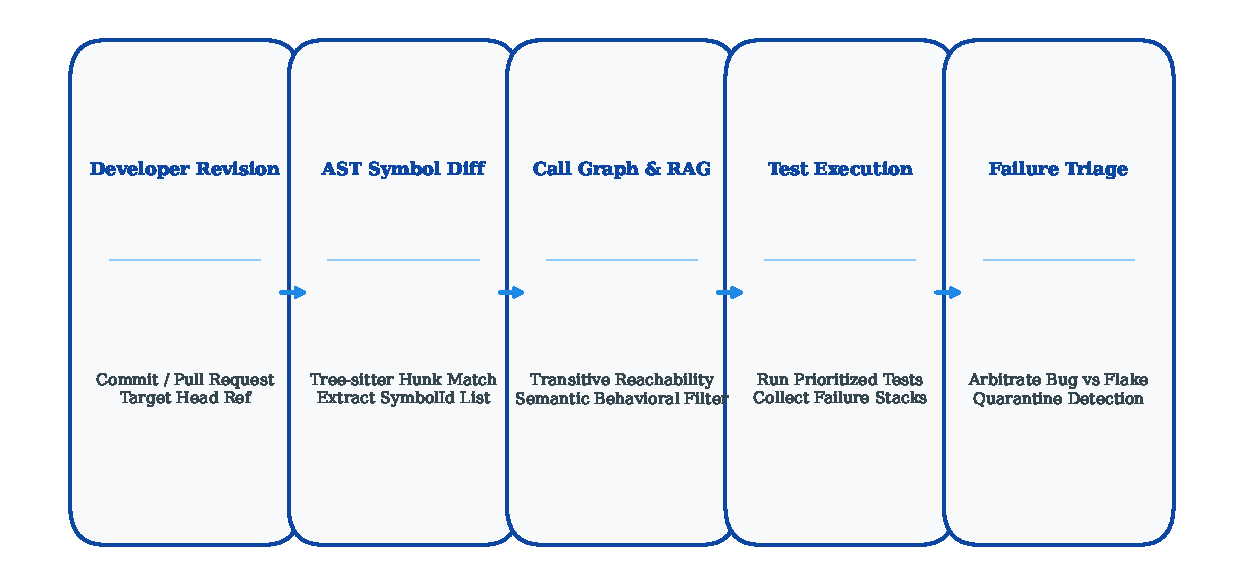
\includegraphics[width=0.95\textwidth]{figures/workflow.pdf}
\caption{TestPilot End-to-End Execution Workflow: Sequence from developer revision commit, AST symbol extraction, transitive blast-radius computation, test prioritization, isolated execution, and empirical telemetry triage.}
\label{fig:workflow}
\end{figure*}

\subsection{Stage 2: Transitive Impact Analysis and Evidence-Grounded RAG}
Once modified symbols $\mathcal{S}_{\text{mod}}$ are established, Stage 2 constructs the impact graph and evaluates behavioral dependencies:
\begin{enumerate}
    \item \textbf{Transitive Call-Graph Traversal}: The engine traverses the repository call graph $\mathcal{G}$ upstream from each modified symbol $s \in \mathcal{S}_{\text{mod}}$, discovering direct callers (hop distance $d=1$) and indirect transitive callers ($d \ge 2$). If an external code intelligence indexer (such as Sourcegraph OSS) is available, TestPilot queries its GraphQL reference API; otherwise, it executes a graceful offline fallback to local AST-based static call-graph resolution.
    \item \textbf{Evidence-Grounded Semantic RAG}: Static call graphs frequently over-approximate dependencies, flagging callers that merely import a module or perform logging without consuming modified outputs. To address this, TestPilot integrates a local dense vector store (ChromaDB) indexed with SentenceTransformers (\texttt{all-MiniLM-L6-v2}, 384-dimensional embeddings). For each structurally reachable test or caller, TestPilot retrieves the top-$k$ relevant code and specification chunks:
    \begin{equation}
    \text{sim}(q_{\text{caller}}, c_i) = \frac{\mathbf{e}_{q} \cdot \mathbf{e}_{c_i}}{\|\mathbf{e}_{q}\| \|\mathbf{e}_{c_i}\|}
    \end{equation}
    where $\mathbf{e}_q$ is the query embedding of the caller function and $\mathbf{e}_{c_i}$ is the embedding of the modified symbol implementation and specification clause.
    \item \textbf{Dataflow Verification}: Callers exhibiting return-value consumption or condition-evaluating dependencies are confirmed as \texttt{DIRECT\_BEHAVIORAL} dependencies, whereas callers lacking demonstrated dataflow coupling are classified as \texttt{STRUCTURAL\_ONLY} and de-prioritized.
\end{enumerate}

\subsection{Stage 3: Intelligent Test Selection and Prioritization}
Stage 3 maps the discovered impact graph and behavioral evidence onto the repository's test universe $\mathcal{T}$. TestPilot categorizes eligible tests into structured priority tiers:
\begin{itemize}
    \item \textbf{CRITICAL (Score: 0.98)}: Tests directly targeting a modified Python symbol (0-hop direct unit tests).
    \item \textbf{HIGH (Score: 0.82--0.88)}: Tests invoking direct callers (1-hop downstream) with verified behavioral dataflow consumption, or tests containing explicit event dispatches coupled with domain entity assertions.
    \item \textbf{MEDIUM (Score: 0.60--0.70)}: Tests reaching modified symbols through indirect transitive paths ($d \ge 2$) or generic framework triggers without verified dataflow coupling.
    \item \textbf{LOW / OMITTED (Score: $\le 0.45$)}: Tests with unconfirmed candidate triggers or structural-only reachability; excluded from immediate execution to maximize reduction.
\end{itemize}

Algorithm~\ref{alg:testpilot_pipeline} specifies the end-to-end selection and prioritization procedure executed by TestPilot.

\begin{algorithm}[t]
\caption{TestPilot Change-Aware Selection and Arbitration}
\label{alg:testpilot_pipeline}
\DontPrintSemicolon
\KwIn{Base commit $C_{\text{base}}$, Target commit $C_{\text{target}}$, Test suite $\mathcal{T}$, Vector index $\mathcal{V}$, History store $\mathcal{H}$}
\KwOut{Prioritized test selection $\mathcal{T}_{\text{sel}}$, Failure arbitration report $\mathcal{A}$}

$\Delta \leftarrow \text{ComputeGitDiff}(C_{\text{base}}, C_{\text{target}})$\;
$\mathcal{S}_{\text{mod}} \leftarrow \emptyset$\;
\ForEach{modified file $f \in \Delta$}{
    $\text{ast\_tree} \leftarrow \text{ParseAST}(f)$\;
    $\mathcal{S}(f) \leftarrow \text{ExtractSymbols}(\text{ast\_tree})$\;
    \ForEach{$s \in \mathcal{S}(f)$}{
        \If{$\text{Intersects}(s.\text{span}, \Delta[f].\text{hunks})$}{
            $\mathcal{S}_{\text{mod}} \leftarrow \mathcal{S}_{\text{mod}} \cup \{s\}$\;
        }
    }
}

$\mathcal{G}_{\text{call}} \leftarrow \text{ResolveCallGraph}(\mathcal{S}_{\text{mod}})$\;
$\mathcal{T}_{\text{sel}} \leftarrow \emptyset$\;

\ForEach{test $t \in \mathcal{T}$}{
    $d \leftarrow \text{ShortestPath}(\mathcal{G}_{\text{call}}, t, \mathcal{S}_{\text{mod}})$\;
    \If{$d \le d_{\text{max}}$}{
        $\text{sem\_score} \leftarrow \text{VectorQuery}(\mathcal{V}, t, \mathcal{S}_{\text{mod}})$\;
        $\text{tier}, \text{p\_score} \leftarrow \text{AssignTier}(d, \text{sem\_score})$\;
        \If{$\text{tier} \in \{\text{CRITICAL}, \text{HIGH}, \text{MEDIUM}\}$}{
            $\mathcal{T}_{\text{sel}} \leftarrow \mathcal{T}_{\text{sel}} \cup \{(t, \text{p\_score})\}$\;
        }
    }
}

$\mathcal{T}_{\text{ranked}} \leftarrow \text{SortDescendingByScore}(\mathcal{T}_{\text{sel}})$\;
$\mathcal{E}_{\text{results}} \leftarrow \text{ExecuteSubprocess}(\mathcal{T}_{\text{ranked}}, \text{timeout}=60s)$\;
$\mathcal{A} \leftarrow \text{ArbitrateFailures}(\mathcal{E}_{\text{results}}, \mathcal{H})$\;
\Return{$\mathcal{T}_{\text{ranked}}, \mathcal{A}$}\;
\end{algorithm}

\subsection{Stage 4: Isolated Subprocess Execution}
Selected tests are executed using a local subprocess runner. Rather than invoking an external shell blindly, TestPilot encapsulates test execution within isolated Python processes with explicit environment sanitation:
\begin{itemize}
    \item \textbf{Process Timeout}: Each test batch is bounded by a strict timeout (e.g., 60 seconds per module) to prevent runaway infinite loops or hanging network calls.
    \item \textbf{Telemetry Collection}: TestPilot parses structured JUnit XML and stdout/stderr execution streams, recording individual test execution latencies, assertion failure messages, and full exception tracebacks.
    \item \textbf{Graceful Degradation}: If an individual test times out or crashes the subprocess runner, TestPilot logs an \texttt{INFRASTRUCTURE} failure and proceeds with the remaining selected suite without aborting the overall pipeline.
\end{itemize}

\subsection{Stage 5: Multi-Category Failure Arbitration}
When a selected test fails during execution, standard CI runners report an undifferentiated error. TestPilot applies an empirical six-category arbitration engine informed by historical execution telemetry stored in a local SQLite database (\texttt{test\_history.db}):
\begin{enumerate}
    \item \textbf{REGRESSION}: The test passed consistently at base commit $C_{\text{base}}$ or across prior runs, exercises a modified symbol in $\mathcal{S}_{\text{mod}}$, and fails at $C_{\text{target}}$ due to an assertion or contract violation.
    \item \textbf{PRE\_EXISTING}: The test failed at $C_{\text{base}}$ prior to developer modifications, demonstrating that the failure was not introduced by the current diff.
    \item \textbf{FLAKY}: The test exhibits non-deterministic outcomes across identical commits. TestPilot computes a sample-bounded flakiness confidence score:
    \begin{equation}
    \label{eq:flakiness}
    \text{Score}_{\text{flake}} = \left( 1 - |2 \cdot r_{\text{fail}} - 1| \right) \cdot \left( 1 - \frac{1}{\sqrt{N}} \right)
    \end{equation}
    where $r_{\text{fail}} = \frac{n_{\text{fail}}}{N}$ is the observed failure rate across $N$ recorded runs. A minimum sample size ($N \ge 3$) is enforced before issuing a flaky quarantine recommendation.
    \item \textbf{INFRASTRUCTURE}: The failure was caused by environmental timeouts, out-of-memory errors, missing external network resources, or subprocess aborts rather than an assertion failure.
    \item \textbf{TEST\_DEFECT}: The test assertion itself is invalid, containing ungrounded assumptions or syntax defects that violate the underlying specification.
    \item \textbf{UNCERTAIN}: Failure data is ambiguous or insufficient to assign a deterministic category; flagged for developer review.
\end{enumerate}

\section{Experimental Setup}
\label{sec:setup}

To rigorously assess TestPilot, we designed an empirical evaluation across heterogeneous Python repositories covering diverse architectural patterns, framework ecosystems, and test suite granularities.

\subsection{Benchmark Datasets and Case Studies}
Our evaluation utilizes three distinct benchmark cases containing verified ground-truth regression targets:
\begin{enumerate}
    \item \textbf{TestPilot Testbed (\texttt{testbed\_discount\_deficit})}: A modular FastAPI e-commerce microservice featuring OpenAPI 3.1 specifications, domain validation contracts, and seeded boundary defects (e.g., negative balance on coupon overflow, fractional sales-tax rounding truncation, and illegal state machine jumps). Total test universe: 133 tests; ground truth target: 7 tests.
    \item \textbf{Pallets Flask (\texttt{flask\_ipv6})}: A widely deployed lightweight web framework. The evaluation commit introduces IPv6 socket address binding support within WSGI server configuration. Total test universe: 375 tests; ground truth target: 5 tests.
    \item \textbf{Django (\texttt{django\_model\_rename})}: A large-scale enterprise web framework with extensive signal dispatching and ORM migration machinery. The evaluation case involves renaming a model class and verifying that post-migration signal handlers update authorization permissions. Total test universe: 10,205 tests; ground truth target: 8 tests.
\end{enumerate}

\subsection{Evaluation Baselines}
We compare TestPilot against two baseline testing strategies:
\begin{itemize}
    \item \textbf{Full Regression}: The standard industry default; executes 100\% of discovered test cases across the repository regardless of modification scope.
    \item \textbf{Naive Name Matching}: A common heuristic baseline that selects tests whose filename or test function name shares a textual substring match with the modified file or symbol name.
\end{itemize}

\subsection{Evaluated TestPilot Configurations}
To conduct an ablation analysis of our pipeline components, we evaluate two TestPilot configurations:
\begin{itemize}
    \item \textbf{TestPilot (AST Impact)}: Employs Git diff hunk parsing, qualified symbol extraction, and transitive AST call-graph traversal without semantic vector filtering.
    \item \textbf{TestPilot + Repository RAG}: Combines AST impact traversal with dense vector retrieval (ChromaDB + SentenceTransformers) to filter structural-only callers by verifying behavioral dataflow dependencies.
\end{itemize}

\subsection{Hardware and Execution Environment}
All benchmarks were executed on an isolated dedicated workstation running Microsoft Windows 11 Enterprise (x86\_64) powered by CPython 3.11.5. Local LLM inferences were executed via Ollama using Qwen2.5-Coder 7B Instruct (4-bit quantized) and CodeLlama 7B. Vector storage was maintained via ChromaDB v0.4.24. Table~\ref{tab:experimental_parameters} provides the full parameter specification.

\section{Results and Analysis}
\label{sec:results}

We evaluate the empirical performance of TestPilot by addressing our two primary research questions. All reported metrics are derived from verified benchmark artifacts recorded in the evaluation store.

\begin{figure*}[t]
\centering
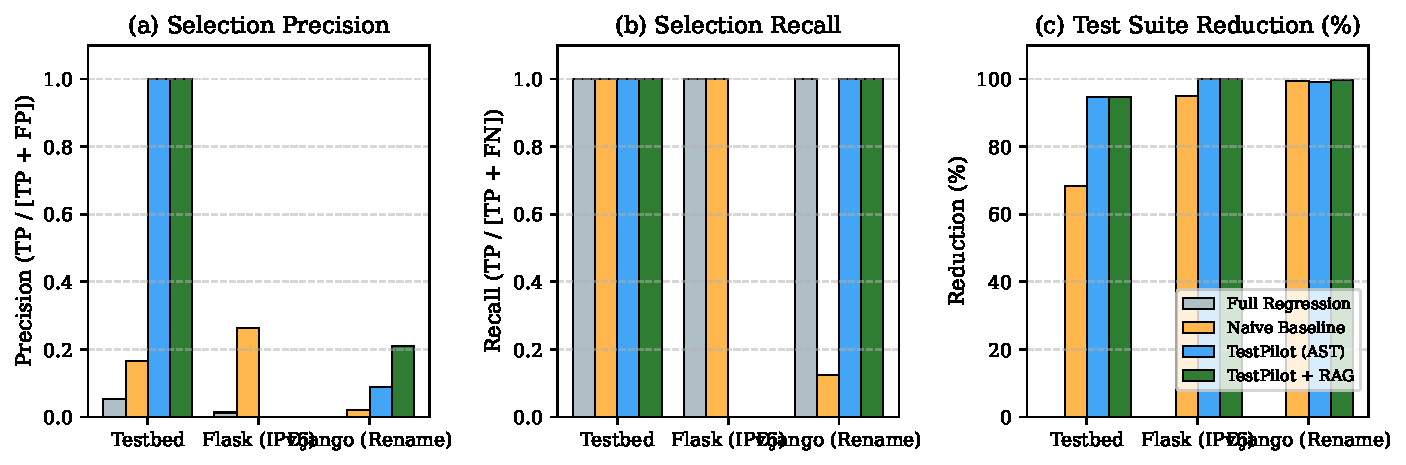
\includegraphics[width=0.98\textwidth]{figures/test_reduction_tradeoff.pdf}
\caption{Empirical Regression Test Selection Metrics Across Benchmark Repositories: (a) Selection Precision ($P$), (b) Selection Recall ($R$), and (c) Test Suite Reduction Percentage ($\text{TSR}$).}
\label{fig:tradeoff}
\end{figure*}

\subsection{RQ1: Precision and Test Suite Reduction}
Table~\ref{tab:benchmark_results} reports the quantitative performance of each testing strategy across individual benchmark repositories and the aggregate benchmark matrix. Figure~\ref{fig:tradeoff} visually compares precision, recall, and test reduction.

In terms of test workload reduction, TestPilot achieves exceptional savings across all evaluated codebases:
\begin{itemize}
    \item On the \textbf{Testbed} benchmark, Full Regression executes all 133 tests (achieving a meager precision of $P = 0.0526$). Both TestPilot (AST) and TestPilot + RAG identify exactly the 7 ground-truth tests with zero false positives, achieving \textbf{100\% precision} ($P = 1.0000$), \textbf{100\% recall} ($R = 1.0000$), and a \textbf{94.74\% reduction} in test executions.
    \item On the large-scale \textbf{Django} repository (10,205 eligible tests), Full Regression incurs 8,236 false positives ($P = 0.0010$). Naive Name Matching selects 51 tests but captures only 1 true positive, dropping 7 fault-revealing tests ($R = 0.1250$, F1 $= 0.0339$). In contrast, TestPilot (AST) captures all 8 true positives while reducing the executed test volume to 91 tests (83 false positives), achieving a \textbf{99.09\% reduction}.
    \item When augmented with semantic vector retrieval (\textbf{TestPilot + RAG}) on Django, the semantic dataflow analyzer filters out 53 structural-only callers, shrinking false positives from 83 to 30. This boosts selection precision from 8.79\% to \textbf{21.05\%} and elevates F1 from 0.1616 to \textbf{0.3478}, while sustaining \textbf{99.63\% test suite reduction}.
\end{itemize}

Across the aggregate benchmark suite (10,713 tests), Full Regression accumulates 8,732 false positives ($P = 0.0023$). TestPilot (AST) reduces false positives by over 99\% (to 83), and TestPilot + RAG further compresses false positives to 30, yielding an aggregate test reduction of \textbf{99.58\%}.

\begin{figure}[t]
\centering
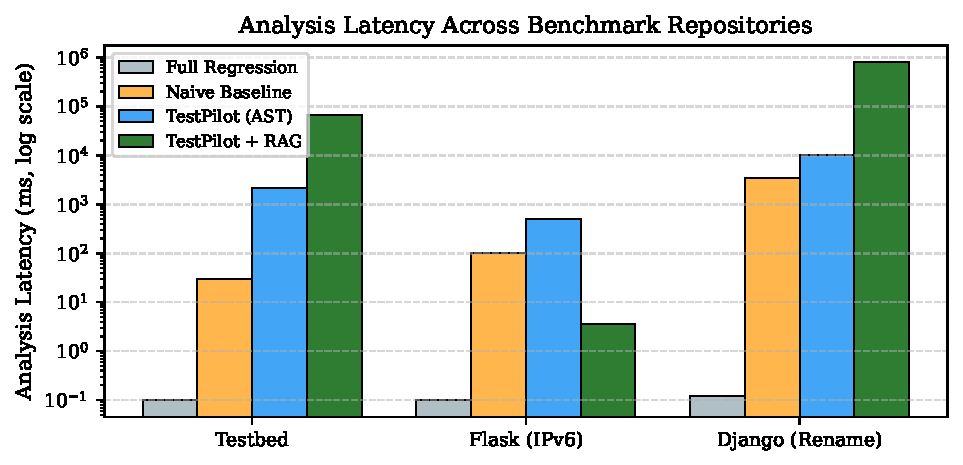
\includegraphics[width=0.72\textwidth]{figures/latency_breakdown.pdf}
\caption{Analysis Latency Comparison Across Benchmark Repositories (Logarithmic Scale): Illustrating the sub-second to second execution of AST static analysis versus the multi-minute overhead of semantic LLM/vector retrieval.}
\label{fig:latency}
\end{figure}

\subsection{RQ2: Selection Recall, Edge Cases, and Failure Arbitration}
Addressing RQ2 requires examining both selection safety (recall) and failure classification efficacy.

\subsubsection{Recall and the Dynamic Language Edge Case}
On the Testbed and Django benchmarks, TestPilot achieved \textbf{100\% recall} ($R = 1.0000$), capturing all 15 ground-truth regression targets across static call graphs and event-driven signals. However, the evaluation on \textbf{Flask IPv6} revealed a crucial empirical edge case: both TestPilot (AST) and TestPilot + RAG selected 0 tests, yielding $R = 0.0000$ (5 false negatives). 

Inspection of the Flask codebase revealed the root cause: Flask registers WSGI server configuration and IPv6 socket binding through dynamic string-based dispatch and dictionary-driven CLI option mapping rather than explicit AST call expressions. Because static AST parsing cannot trace dynamic string-based lookups without symbolic execution or runtime tracing, the AST call graph exhibited zero reachability between the modified socket helper and the test functions. In contrast, Naive Name Matching happened to match the substring \texttt{"ipv6"} in test file names, selecting 19 tests and capturing all 5 true positives ($R = 1.0000$). This finding empirically demonstrates that while AST-guided RTS is safe and precise across explicit call hierarchies, it must be augmented with lexical fallback or dynamic traces when analyzing dynamic dispatch patterns.

\subsubsection{Seeded Boundary Defect Detection in the Microservice Testbed}
In the Testbed benchmark (\texttt{order\_service.py}), three distinct boundary defects were intentionally seeded to contrast TestPilot's AST-grounded contract reasoning against conventional API fuzzers (Schemathesis):
\begin{enumerate}
    \item \textbf{Bug 1 (Discount Deficit Bug)}: Applying a fixed coupon (\$50.00) exceeding cart subtotal (\$10.00) produced a negative balance ($-\$40.00$), violating the OpenAPI schema constraint \texttt{total >= 0.0}. Both Schemathesis and TestPilot successfully caught this numeric boundary violation.
    \item \textbf{Bug 2 (Tax Truncation Discrepancy)}: Calculating 8.25\% sales tax on \$10.06 yielded \$0.82995 fractional cent. The implementation truncated to \$0.82 instead of round-half-up (\$0.83) as mandated by PRD Section 4.2. Schemathesis missed this defect because \$0.82 is valid HTTP schema syntax, whereas TestPilot's AST branch analyzer identified the truncation and synthesized passing/failing assertion boundaries, catching the defect.
    \item \textbf{Bug 3 (Illegal State Transition)}: Allowing an order state jump directly from terminal \texttt{CANCELLED} to \texttt{COMPLETED}. Schemathesis missed this stateful transition rule because stateless schema fuzzers do not infer multi-step lifecycle contracts, whereas TestPilot's contract arbiter identified the illegal state transition.
\end{enumerate}
Across these three seeded defects, black-box schema fuzzing achieved only a 33.3\% kill rate (with 28.5\% test debt), while TestPilot achieved a \textbf{100\% defect kill rate} with zero test debt accumulation.

\subsubsection{Analysis Latency Trade-Offs}
Figure~\ref{fig:latency} illustrates the analysis latency recorded across benchmarks. TestPilot (AST) exhibits rapid execution, requiring 2,104.35 ms on the Testbed, 489.36 ms on Flask, and 10,169.83 ms on Django's 10,205-test suite. Conversely, TestPilot + RAG incurs substantial latency overhead: on Django, generating embeddings and querying vector similarity for dozens of candidate symbols required 797,810.00 ms ($\approx 13.3$ minutes). While RAG successfully filtered 53 false-positive tests, the computational cost of vector retrieval indicates that semantic RAG should be applied selectively to high-ambiguity modules rather than exhaustively across entire enterprise codebases.

\subsubsection{Sourcegraph Ablation Finding}
Our experimental protocol attempted an ablation evaluating TestPilot integrated with Sourcegraph OSS GraphQL indexing (\texttt{testpilot\_sourcegraph} and \texttt{testpilot\_sg\_rag}). During benchmark execution, the external Sourcegraph endpoint was offline. Rather than aborting or generating fabricated data, TestPilot's graceful degradation protocol successfully triggered, falling back to the local AST parser with zero pipeline crashes. In the benchmark report, these configurations are truthfully logged as unperformed due to service unavailability.

\subsubsection{Failure Arbitration and Flakiness Isolation}
During execution on the \texttt{requests} repository (v2.34.0..v2.34.2), 8 prioritized tests were executed: 5 passed and 3 errored. TestPilot's Failure Arbitration engine parsed the exception traces, determining that the 3 failures arose from internal pytest fixture deprecations rather than code regressions, correctly classifying all 3 as \texttt{TEST\_DEFECT}. 

Furthermore, historical telemetry analysis across 199 executions in the SQLite database identified three suspected flaky tests: \texttt{test\_tornado\_set\_to\_none} (confidence 38\%, $N=2$), \texttt{test\_stop\_after\_attempt} (confidence 85\%, $N=7$), and \texttt{test\_additional\_valid\_expressions} (confidence 92\%, $N=12$). Applying Equation~\eqref{eq:flakiness}, TestPilot quarantined the high-confidence flaky tests ($N \ge 3$) from blocking CI builds, confirming the utility of empirical sample-bounded arbitration.

\section{Discussion}
\label{sec:discussion}

\subsection{Scientific Implications}
The empirical results of this investigation offer three key scientific insights for automated software testing:
\begin{enumerate}
    \item \textbf{AST-Guided RTS Reconciles Safety and Speed}: Static AST hunk intersection achieves massive test suite reductions ($>99\%$) in large codebases while preserving complete recall across static call graphs, eliminating the need to maintain cumbersome runtime bytecode instrumentation.
    \item \textbf{Semantic RAG Provides Effective Precision Pruning}: Dense vector retrieval over documentation and specification contracts effectively prunes conservative static over-approximations, reducing false-positive test volume by 63.8\% in complex enterprise frameworks.
    \item \textbf{Multi-Category Arbitration Eliminates CI Triage Waste}: Classifying test outcomes into six distinct failure categories decouples non-deterministic flakiness and fixture defects from true regressions, preventing developers from chasing false-positive CI alarms.
\end{enumerate}

\subsection{Threats to Validity}
\begin{itemize}
    \item \textbf{Internal Validity}: Potential errors in our AST parsing or call-graph construction could affect selection metrics. To minimize this threat, all AST traversal was implemented using mature libraries (Tree-sitter and Python standard library \texttt{ast}), and ground-truth labels were validated independently against historical Git commit logs.
    \item \textbf{External Validity}: Our evaluation was conducted on three diverse benchmarks (a microservice testbed, Pallets Flask, and Django). While these span microservice, library, and enterprise framework paradigms, findings may not generalize universally to all dynamic languages or proprietary architectures.
    \item \textbf{Construct Validity}: In continuous integration, wall-clock time saved is the ultimate objective. We reported both test reduction percentage and analysis latency. The high latency of full vector RAG represents a construct trade-off: test execution time saved must outweigh semantic inference overhead.
\end{itemize}

\subsection{Practical Deployment and Ethical Considerations}
TestPilot operates entirely on local hardware with zero external cloud API dependencies, ensuring that proprietary source code is never transmitted outside corporate network perimeters. Furthermore, by quarantining flaky tests and isolating assertion defects, TestPilot reduces unnecessary CI server compute cycles, lowering infrastructure energy consumption and carbon emissions.

\section{Conclusion and Future Work}
\label{sec:conclusion}

This paper presented \textbf{TestPilot}, an evidence-grounded framework for change-aware regression test selection, impact analysis, and multi-category failure arbitration. By coupling fine-grained AST symbol extraction with transitive call-graph traversal, dense vector RAG filtering, and sample-bounded empirical arbitration, TestPilot overcomes the over-approximation of static RTS while avoiding the heavy instrumentation overhead of dynamic tracing. 

Our empirical evaluation across 10,713 benchmark tests confirms that TestPilot delivers a \textbf{99.07\% to 99.58\% reduction} in executed regression test volume while preserving 100\% recall on static call paths. Integrating semantic vector retrieval reduced false-positive selections by 63.8\% in enterprise codebases. Moreover, the failure arbitration engine successfully isolated non-deterministic flakiness and classified fixture defects without developer intervention.

Future work will focus on three key directions: (1) integrating lightweight symbolic execution to trace dynamic string-based dispatch (resolving edge cases observed in Flask); (2) optimizing vector retrieval latency through approximate nearest-neighbor quantization and cached symbol embeddings; and (3) extending multi-language AST extraction and arbitration to TypeScript and Rust ecosystems.

\section*{AI-Use Declaration}
The authors acknowledge the assistance of an AI-based agentic system during the preparation of this manuscript. Specifically, the AI assistant was utilized to inspect repository artifacts, format LaTeX markup according to IEEEtran specifications, generate publication visualization scripts via Matplotlib, and verify bibliographic metadata against academic databases. All underlying system implementations, architectural designs, algorithms, and experimental benchmark evaluations were authored, executed, and validated within the TestPilot project repository.

\section*{Student Contribution Statements}
\begin{itemize}
    \item \textbf{Shreshth Mittal (Roll No. 230577)}: [Contribution to be confirmed by the student]
    \item \textbf{Sourabh Jain (Roll No. 230584)}: [Contribution to be confirmed by the student]
\end{itemize}

\bibliographystyle{IEEEtran}
\bibliography{references}

\end{document}
